\chapter{Related Work}

\section{Acoustic Array Design}
\subsection{Heupel et al - Automated acoustic tracking of aquatic animals: scales, design and deployment of listening station arrays}
In their highly cited 2006 publication\cite{Heupel2006}, Heupel et al discuss issues and methods related to the implementation of acoustic tracking network.  They list the small size, low cost, and low maintenance requirements as primary drivers of the technology's popularity within the biological community.  The authors point out that lower cost of acoustic instruments facilitates larger sample sizes and datasets.  Additionally, because acoustic tracking is a passive process (researchers need not actively follow tagged animals to collect telemetry), data can be collected around the clock, while active tracking expeditions would be limited by inclement weather.  Furthermore, because animals are not being shadowed by a noisy vessel, they are more likely to exhibit natural behavioral patterns.\newline
\newline
The authors discuss the importance of identifying study goals, and using those goals to drive array design.  If high-resolution, positional accuracy is important, an array with high levels of overlapping receivers will allow for triangulation of a tag within 3D space.  Animal residency within a specific area can be assessed with a "curtain" or "gate" (parallel lines of receivers around the area of interest) of receivers that will track animal ingress and egress.  Presence/absence tracking and long-term survivorship can be can both be accomplished established by a sparse (dispersed) array of receivers, as only occasional transmissions are necessary to address questions of this nature.\newline
\newline
Heupel et al offer a plethora of practical advice for implementing acoustic arrays, such as how to assemble acoustic rigs and environmental phenomena that affect the propagation of acoustic signals.  Environmental impedances to acoustic signal propagation include: background noise, composition of the sea floor, thermoclines and pycnoclines , salinity, and tidal flows.  Other factors are less obvious, such as the positioning of the receiver in regards to the rigging (is any part of the rigging creating an acoustic shadow?), signal collision due to echoes and presence of multiple tags, and the development of fouling organisms on the receiver.  The authors suggest that extensive field testing should be done prior to the commencement of any acoustic study.


\subsection {Steel et al - Performance of an ultrasonic telemetry positioning system under varied environmental conditions}
In 2014, Steel et al\cite{Steel2014} investigated the accuracy of the VEMCO Positioning System (VPS), comparing its accuracy to GPS, and investigating possible sources of inaccuracy.  VPS is a VEMCO proprietary service that uses data gathered from multiple VEMCO acoustic receivers and uses triangulation to "fix" (determine) the position of a tag.  To generate data, acoustic tags were deployed as permanent emplacements (with known GPS coordinates) throughout the study site, and VPS fixes were compared against known GPS coordinates using Euclidian distance to find the "Horiziontal Positional Error in meters" (HPEm).  The study also tracked "Positional Efficiency", as the percentage of pings a receiver captured.  The study was performed in river, estuary, and coastal locations.  Environmental variables were measured throughout the study, and included wind, wave period, wave height, water temperature, flow, turbidity, electrical conductivity, macrophyte growth rate, and discharge.  The only user-controlled variable was the array geometry.  Generalized Linear Mixed Modeling showed that both Positional Efficiency and HPEm were most strongly correlated with position within the network.  Specifically, tags in the center of the network had the smallest HPEm values, and the lowest positional efficiency.  This makes sense as tags placed in the middle of the network were observed by many more receivers than those on the outskirts of the array.  At the same time, tags in the middle of the array were probably receiving acoustic interference form neighboring tags, which likely caused destructive transmission interference.  Tags on the outskirts of the array had fewer neighbors, and so likely less interference.  The authors concluded that array geometry was the most important predictor of positioning performance. They suggest that field testing both array geometries and environmental conditions is an important step in acoustic tracking studies.



\subsection{Kessel et al - Close proximity detection interference with acoustic telemetry: the importance of considering tag power output in low ambient noise environments}
In their 2015 publication, Kessel et al\cite{Kessel2015} discuss how acoustic transmission power affects acoustic reception.  The team denounces a popular misconception that "higher tag power is better" by presenting evidence of Close Proximity Detection Interference (CPDI).  While most researchers are concerned with the increasing the maximum detection range of their acoustic tags, they rarely ever consider the effect of increased transmission power at close range.  To investigate the properties of CPDI, the authors conducted range testing in three distinct acoustic environments: (a)Cumberland sound, Baffin Island, Nunavut, Canada, (b)Lake Charlotte, Nova Scotia, Canada, and (c)Jupiter, Florida, USA.  Range testing was done by deploying acoustic receivers (VEMCO VR2W 69kHz) and acoustic tags (V16-6H and V13-2H) at varying distances.  Table~\ref{CPDItable} lists the pyhsical characteristics of each study site.

\begin{table}[h!]
	\begin{tabular}{l l l l l}
		Location&Depth&Receiver Elevation&Sea floor composition\\
		\hline
		Lake Charlotte			& 40m	& 5m	& hard seafloor \\
		Cumberland sound		& 30m	& 3m	& soft mud	\\
		Jupiter, Florida		& 20m	& 2m	& 1.5m of sand over hard reef\\
	\end{tabular}
	\caption{Study Site Characteristics}
	\label{CPDItable}
\end{table}

\begin{table}[h!]
	\begin{tabular}{l l l l l}
		Tag	&Range	&Detection \%	&Range	&Detection \%\\
		\hline
		V16-6H	&55m	& 8.3 \%		&370m	&88.8 \%\\
		V13-2H	&55m 	& 17.9 \%	&221m	&88.4 \%\\
	\end{tabular}
	\caption{Cumberland Sound Range Test Data}
	\label{rangeTestData}
\end{table}

The team observed that tags very close to a receiver had relatively low detection rates (Table~\ref{rangeTestData}).  The team notes a "Donught" shaped zone of poor reception around a receiver.  At Cumberland sound, the team noted a strong CPDI effect, likely due to the hard sea floor, and low wind/wave action.  At Lake Charlotte, the team recorded more pings than were released, indicating that acoustic echoes were being recorded in addition to primary transmissions.   They also noted a reduced number of transmissions during periods of very high wind.  At Jupiter, Florida, the team found the weakest CPDI effect, accrediting it to the sandy bottom, reef structure, and noisy (wind, wave, boating activity \& fauna) environment.  They concluded that at close range, transmissions echo off the surface and sea floor, interfering with reception of the primary transmission.  At greater ranges, the strength of these echoes drop off, and the primary transmission becomes the dominant signal.  The team noted that hard surfaces likely promoted the echoing of transmissions, while softer sediment helps to absorb them.  They also point out that strong wind likely caused surface distortions, which reduced the potential for acoustic reflection.  Finally, background noise (such as that of human water activity, wave action, and marine fauna) helped to reduce CPDI, but decreased the maximum detection range.


\section{Sensor Placement Algorithms}
\subsection{Howard et al - Mobile Sensor Network Deployment using Potential Fields Potential Field Algorithm}
In 2002, Howard et al described an algorithm for the autonomous dispersion of a mobile sensor network in an unknown environment.  Their model described each sensor a point charge that repelled other sensors and walls.  At each iteration of the simulation, sensors pushed and pulled against each other, resulting in a net vector for that iteration.  The simulation was iterated until all sensor movement ceased.  A small static force allowed for the cessation of endless fine-scale movements and termination the simulation.  The team found that by letting this simulation "settle", an optimal or near-optimal coverage solution could be found.  


\subsection{Poduri et al – Constrained Coverage for Mobile Sensor Networks Constrained Coverage (K-Neighbor Networks vs Maximum Coverage)}
In their 2004 paper, Poduri et al\cite{Poduri2004} expand upon the concept presented by Howard-et-al \cite{Howard2002}, describeing an algorithm for maximizing the sensor coverage of an enclosed space while maintaining the property that each sensor has at least k-neighbors. Just as in Howard et al's work, the team's approach utilized a force dispersion algorithm where each sensor represented a point force, pushing against other nodes to extend coverage.  To satisfy the k-neighbor requirement, sensors exhibited a strong attraction towards other nodes that had fewer than k-neighbors.  The simulation settled when the k-neighbor requirement was satisfied for all nodes.  

With respect to acoustic tracking networks, this approach is useful in fine-scale movement tracking where maintaining the ability to triangulate tag positions is key.  However, this approach tends to require a large number of sensors relative to the size of the study area.  Small sensor to space ratios (only a few sensors for a very large area) would likely find that the k-neighbor network, while providing high-resolution tracking, covered too small of an small area.


\subsection{Akbarzadeh et al - Probabilistic Sensing Model for Sensor Placement Optimization Based Signal Simulation and Attenuation (Omni Directional Sensors)}
In their 2013 paper, Akbarzadeh et al\cite{Akbarzadeh2013} discuss the optimization of sensor coverage using probabilistic detection and attenuation models.  Within the context of a wireless sensor network composed of small devices with limited, directed sensing capabilities, they discuss finding minimal sensor placements such that areas of interest are covered.  In their model, sensors had a limited degree of vision, requiring optimization of both sensor 3D placement and angle.  The definition of coverage followed a probabilistic model, where sensors were subject to attenuation due to distance and obstruction (due to physical objects and environmental factors).  The authors claimed that the omni-directional "disc" model for sensor coverage led to highly inflated coverage values.  They also contend that a 2D x/y model is unrealistic, and that sensor placements should fall into a 3D space, where sensors can be placed at varying heights to achieve optimal coverage.  They give the example of video surveillance in an urban environment, where certain areas of interest require sensor (camera) coverage, are subject to obstruction, and attenuation (difficult to make out images from far away).  In this model, they attempt to find optimal 3D placements of sensors and sensor angles to achieve the required coverage with a minimal number of sensors. 

They also present a model for determining Line of Sight based on a gridded 3D system.  Within this system, a 2D grid of elevations represents 3D space as solid rectangular prisms.  The left panel of Figure\ref{rayTracingImg} shows how ray tracing is used to determine which cells potentially block the line of sight between the sensor-contating cell $p$, and the target cell $q$.  In the right panel, shaded cells must be evaluated to determine the portion of the target area in $q$ is visible from $p$.
\begin{figure}[t]
	\label{rayTracingImg}
	\centering
	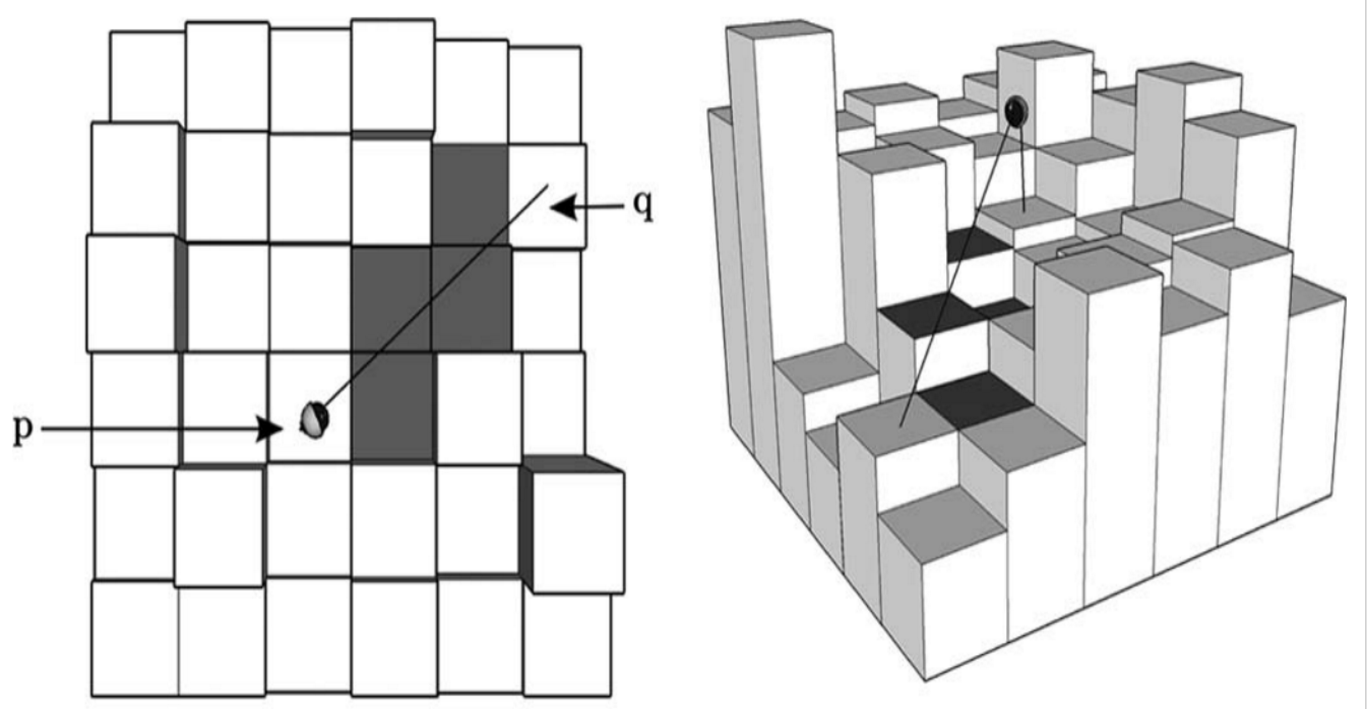
\includegraphics[scale=0.3]{rayTracing.png}
	\caption{An illustration of how ray tracing is used within a 3D environment to identify potential visual obstructions.  Ray tracing is used to determine which cells potentially block the line of sight between the receiver-contating cell $p$, and the target cell $q$.  Shaded cells must be evaluated by a Line of Sight algorithm to determine the portion of the target area in $q$ is visible from $p$. \cite{Akbarzadeh2013}}
\end{figure}

Our simulation is heavily based upon the probabilistic detection models presented by Akbarzadeh et al.  The attenuation, obstruction, and probabilistic detection models are simplified to model omni-directional acoustic receivers.  Because receivers are omni directional and we assume emplacement a fixed distance off the bottom of the sea floor, we need neither determine the angle of receiver placement, nor the optimal height of receiver placement.  This vastly simplifies our computational complexity, allowing for faster simulation times, and thus iterative designing.


\subsection{Yuan et al - Fast Sensor Placement Algorithms for Fusion-based Target Detection}
The 2008 Yuan et al publication discussed several approaches to maximizing sensor coverage of target areas using the fewest possible sensors.  The defined coverage in terms of the probability of detection $P_d$ and the probability of false positive detections $P_f$.  To be "covered", an area had to have sufficiently high $P_d$ and sufficiently low $P_f$ values.  The team also proposed a probabilistic detection model, where multiple sensors observing the same target could combine their observations via  data fusion to increase $P_d$ and decrease $P_f$ for that target. The model used called for the specification of some number of "target" zones to cover.  The team relied heavily upon a Constrained Simulated Annealing (CSA) algorithm to solve the problem of optimal coverage.  The team found that directly searching for a global optimal solution took exponential time (O(n!)).  The team's second approach utilized a divide and conquer algorithm, which found local solutions for each target area individually, then combined local solutions into a single global solution.  This approach took polynomial time, but resulted in an inefficient global solution.  The authors suggested that, first choosing locations that covered multiple spots, then adding sensors to solve local coverage deficits could improve the algorithm's results.  The final algorithm presented by the team combined a clustering algorithm and the improved divide and conquer strategy.  The clustering algorithm first grouped target locations into larger clusters, then solved for these clusters locally before combining them for a global solution.  This approach both improved the runtime and reduced the total number of required sensors.

The goal of our framework is to recover the greatest number of unique acoustic transmissions given a fixed number of acoustic receivers.  Yuan et al focus on minimizing the number of receivers required to achieve coverage over a given number of target areas.  While their research is very closely related to the goal of our framework, the workflows are fundamentally different.  We believe that SAON designers will more likely find themselves with a finite number of resources to collect as much data as possible (in line with our framework's goal), rather than attempting to achieve specific coverage for target areas.  Still, the ability to address specific coverage requirements is valuable.  Researchers with little knowledge of a target species would likely use our framework, while projects with more refined understandings of their target species would want to utilize Yuan et al's workflow.  


\section{The Economic Value of Information}
\subsection{Hansen \& Jones - The value of Information in Fishery Management}
In their 2008 publication, Hansen \& Jones address the value of information in ecological management through the lens of economic opportunity cost.  In economics, opportunity cost describes the cost of taking a particular action as the value lost by not taking an alternative action.  The authors argue that by investing too heavily in analysis, few resources remain for responsive action.  An underlying assumption is that there is a vast amount of uncertainty in ecology, and that fully realizing the complexities of an ecological system is impossible, no matter how much money is spent attempting to do so.  They also argue that while collecting more information can reduce uncertainty, it is reasonable to assume that there are diminishing returns on the resulting actions (certainty is not linearly correlated with the benefit of the resulting action).  Therefore, they argue that researchers should spend fewer resources on information gathering and more resources on ecological action.  Given fixed research budgets, the opportunity cost of information gathering is then the ecological benefit of action.  

The authors cite two case studies, the first involving the removal of juvenile parasitic sea lampreys from rivers feeding Great Lakes.  Current treatment practices for the project begin by identifying which streams are most in need of treatment, chemically treating those streams, and counting the number of dead juveniles that flow down stream.  The authors note that the cost of analysis (site identification and mortality determination) was nearly a third of the chemical treatment budget.  They argue that by taking an "adaptive" management approach (spending less on data collection and more on treatment), more streams could be treated, leading to a larger ecological impact, despite less accurate assessments.

The second case study was the specification of a global network Marine Protected Areas (MPAs) sufficient to protect the biodiversity and sustainability of fisheries worldwide.  The estimated cost for such a network is 5-19 billion dollars.  The authors claim a mindset exists that MPAs will be more effective if carefully chosen, and that no census exists on where MPAs should be placed. There is little research into correlation of costs for defining MPAs to the effectiveness of the resulting MPA network.  It is believed that a multitude of designs could be "optimal", indicating that suboptimal configurations will result in minimal losses.  The authors claim that all else being equal, spending less on MPA identification, and simply creating more MPAs will reduce the chances of failing to protect a critical location.  Furthermore, the longer it takes to identify MPAs, the more the biodiversity at those sites degrades.  The authors conclude that investments in information gathering should be carefully weighted against other management actions, with the goal of maximizing real-world impacts.

It is important to note that the authors neither excuse nor endorse action without data collection.  Rather, they point out that focusing too many resources on information gathering diminishes ecological impact.  Applying this rationale to our simulation, recreating a perfectly faithful representation of the real world is difficult if not impossible, as there are a great many environmental an physical phenomena that can affect acoustic transmissions.  Modeling all of these phenomena would greatly increase the time and resources necessary to simulate them.  It is important to keep in mind that in practice the framework will likely be used to run several times as researchers tinker with and refine their simulation parameters.  Therefore, an overly complex simulation with a very long run time (hours, days, weeks) could cost many research hours. At the same time, over simplifying a simulation (to the point that it begins omitting significant phenomena) in order to reduce its runtime is a mistake.  If these two "bad" simulations represent the extremes of simulation, then  we contend that a "very good" simulation would consider phenomena that strongly affect the simulation results, and run in a reasonable amount of time.  



